\documentclass[10pt,twocolumn,a4paper]{article}
\usepackage[margin=0.68in,top=0.7in,bottom=0.7in]{geometry}
\usepackage{times}
\usepackage{amsmath,amssymb}
\usepackage{booktabs}
\usepackage{graphicx}
\usepackage{xcolor}
\usepackage{hyperref}
\usepackage{microtype}
\usepackage{caption}
\usepackage{subcaption}
\usepackage{float}

\hypersetup{
    colorlinks=true,
    linkcolor=blue!70!black,
    citecolor=blue!70!black,
    urlcolor=blue!70!black
}

\title{\textbf{Benchmarking Approximate Nearest Neighbour Search: \\ Empirical Trade-offs, Failure Modes, and Mechanistic Analysis}}
\author{
    \textbf{Course: CS4.406 Information Retrieval \& Extraction} \\
    Monsoon Semester 2026
}
\date{}

\begin{document}

\maketitle

\begin{abstract}
Dense retrieval at scale hinges upon high-throughput Approximate Nearest Neighbour (ANN) search. In this work, we conduct a rigorous, single-threaded comparative benchmark of three prominent vector indexing paradigms—Hierarchical Navigable Small World graphs (\textbf{HNSW}), Inverted File Flat (\textbf{IVF-Flat}), and Inverted File Product Quantization (\textbf{IVF-PQ})—against an exact FAISS baseline on \textbf{SIFT-1M} (128D, Euclidean) and \textbf{GloVe-100} (100D, angular). We investigate query latency, memory footprints, and indexing throughput, and evaluate two core failure modes: semantic query difficulty via relative distance contrast on GloVe-100, and the curse of dimensionality under spherical distance concentration on custom synthetic distributions ($d \in [16, 256]$). We demonstrate that while HNSW achieves dominant Pareto throughput on clustered euclidean descriptors, its advantages narrow significantly on semantic hub topologies. Furthermore, we reveal how product quantization imposes a strict structural recall ceiling, and analyze the architectural decision boundary between exact and approximate retrieval under strict memory and latency budgets.
\end{abstract}

\section{Introduction \& Hardware Setup}

Retrieving the $k$ most similar vectors from an $N$-element collection forms the computational bottleneck of contemporary semantic search, recommendation engines, and retrieval-augmented generation (RAG). Exact brute-force scan requires $\mathcal{O}(N \cdot d)$ floating-point operations per query, which becomes prohibitive as $N$ scales into millions. Approximate Nearest Neighbour (ANN) search trades a small fraction of retrieval recall for orders-of-magnitude lower query latency.

\subsection{Experimental Environment}
To eliminate confounding factors such as thread scheduling jitter, NUMA memory migration, and multicore contention, all experiments were conducted in a strictly single-threaded configuration on an isolated physical host.
\begin{itemize}
    \item \textbf{Processor}: Intel(R) Core(TM) i5-1135G7 @ 2.40GHz (4 cores, 8 threads), L1d: 48\,KB, L1i: 32\,KB, L2: 1.25\,MB, L3: 8\,MB.
    \item \textbf{Memory}: 16\,GB DDR4-3200 DRAM.
    \item \textbf{Operating System}: Linux x86\_64 (Kernel 6.16.14).
    \item \textbf{Software Stack}: Python 3.14, FAISS-CPU (1.7.4+), NumPy 1.26+, OpenBLAS backend.
    \item \textbf{Thread Isolation}: Enforced via \texttt{OMP\_NUM\_THREADS=1}, \texttt{OPENBLAS\_NUM\_THREADS=1}, and \texttt{faiss.omp\_set\_num\_threads(1)}.
\end{itemize}

\subsection{Datasets \& Metric Normalization}
We evaluate on two canonical benchmarks from \texttt{ann-benchmarks}:
\begin{enumerate}
    \item \textbf{SIFT-1M}: $1,000,000$ 128-dimensional local image descriptors with Euclidean ($L_2$) distance.
    \item \textbf{GloVe-100}: $1,183,514$ 100-dimensional word vectors trained on Wikipedia/Gigaword under angular (cosine) distance.
\end{enumerate}
Per assignment mandates, GloVe vectors were $L_2$-normalized to the unit sphere: $\mathbf{x}' = \mathbf{x} / \|\mathbf{x}\|_2$. For unit vectors $\mathbf{u}, \mathbf{v} \in \mathbb{S}^{d-1}$, the squared Euclidean distance is monotonically related to angular cosine similarity:
\begin{equation}
    \|\mathbf{u} - \mathbf{v}\|_2^2 = \|\mathbf{u}\|_2^2 + \|\mathbf{v}\|_2^2 - 2 \mathbf{u}^\top \mathbf{v} = 2 - 2 \cos(\mathbf{u}, \mathbf{v})
\end{equation}
Minimizing Euclidean distance over normalized vectors is strictly isomorphic to minimizing angular distance $D_{\text{ang}} = 1 - \cos(\mathbf{u}, \mathbf{v}) = \frac{1}{2} \|\mathbf{u} - \mathbf{v}\|_2^2$.

Queries ($10,000$ total) were partitioned into $5,000$ validation queries (for tuning) and $5,000$ test queries (for final reported metrics).

\section{Part 1: Exact Search Baseline}

\subsection{Custom Recall@10 with Distance Tie-Handling}
In nearest neighbour evaluation, floating-point ties frequently occur at rank $k=10$, particularly when multiple stored items reside at identical distances from a query. Standard set-intersection recall unfairly penalizes arbitrary tie-breaking by the index. 

We implemented a custom metric $\text{Recall}@k$:
\begin{equation}
\small
    \text{Rec}@k(q) = \frac{1}{k} \sum_{i=1}^k \left[ \mathbb{I}(\text{ret}_i \in \text{GT}_k) \lor \mathbb{I}(\text{dist}_i \le D_k(q) + \epsilon) \right]
\end{equation}
where $D_k(q)$ is the distance of the $k$-th ground-truth neighbour, and $\epsilon = 10^{-3}$ accounts for precision tolerances. The metric was validated with unit tests covering permutations, disjoint sets, partial overlaps, and equidistant boundary ties. 

Validating FAISS exact search (\texttt{IndexFlatL2}) against the pre-stored ground truth in the HDF5 datasets yielded \textbf{100.00\% agreement} on both SIFT-1M and GloVe-100.

\subsection{Sequential vs. Batch Query Execution}
We evaluated exact search speed over $5,000$ queries executed sequentially ($1$ query per call) versus in a single batched call ($5,000$ queries simultaneously) on full SIFT-1M and GloVe-100 under single-threaded execution.

\begin{table}[H]
\centering
\small
\caption{Exact Search Baseline Performance (Single Thread)}
\label{tab:exact_baseline}
\resizebox{\columnwidth}{!}{
\begin{tabular}{lcccc}
\toprule
\textbf{Dataset} & \textbf{Mode} & \textbf{Latency (ms)} & \textbf{QPS} & \textbf{Speedup} \\
\midrule
SIFT-1M & Sequential & 12.15 & 82.3 & --- \\
SIFT-1M & Batch & 2.55 & 392.5 & \textbf{4.77$\times$} \\
\midrule
GloVe-100 & Sequential & 11.93 & 83.8 & --- \\
GloVe-100 & Batch & 2.45 & 408.2 & \textbf{4.87$\times$} \\
\bottomrule
\end{tabular}
}
\end{table}

\noindent\textbf{Mechanistic Explanation of the $3.2\times$--$3.3\times$ Speedup}:
\begin{enumerate}
    \item \textbf{BLAS GEMM vs. GEMV Arithmetic Intensity}: Sequential execution evaluates $1$ query against $N$ vectors, executing a Matrix-Vector product (\texttt{GEMV}). GEMV reads $N \times d \times 4$ bytes from memory for only $\mathcal{O}(N d)$ arithmetic operations (intensity $\approx 0.5$ FLOP/byte), stalling on DRAM latency. In contrast, batch execution groups $Q$ queries into a Matrix-Matrix multiplication (\texttt{GEMM}), performing $2 N Q d$ operations over $(N + Q) d$ loaded floats. High arithmetic intensity enables OpenBLAS to tile registers and saturate vector units (AVX2/FMA).
    \item \textbf{Cache Locality \& Memory Bandwidth}: In sequential mode, the entire base matrix ($\approx 500$\,MB) must be re-read from DRAM $5,000$ times. In batch mode, blocks of the database loaded into the L2/L3 cache are simultaneously evaluated across all $Q$ queries, drastically slashing DRAM bus traffic.
    \item \textbf{Call Boundary Overhead}: Batching amortizes $5,000$ individual Python/C++ FFI transitions and per-query memory allocations.
\end{enumerate}

\section{Part 2: Benchmarking HNSW, IVF-Flat, and IVF-PQ}

\subsection{Index Architectures \& Search sweeps}
We benchmarked three representative index families across both datasets:
\begin{itemize}
    \item \textbf{HNSW} (\texttt{IndexHNSWFlat}): Multi-layer proximity graph with build parameters $M \in \{16, 32\}$, $efConstruction \in \{40, 100\}$, and search sweep $efSearch \in [10, 512]$.
    \item \textbf{IVF-Flat} (\texttt{IndexIVFFlat}): Inverted file index with Voronoi coarse quantizer ($nlist \in \{256, 1024, 4096\}$), sweeping search centroids $nprobe \in [1, 128]$.
    \item \textbf{IVF-PQ} (\texttt{IndexIVFPQ}): Inverted file with Product Quantization codes ($nlist=1024$, $m \in \{16, 32\}$ sub-vectors for SIFT, $m \in \{10, 20\}$ for GloVe, 8 bits/code), sweeping $nprobe \in [1, 128]$.
\end{itemize}

Every search timing was evaluated sequentially (1 query at a time) across the $5,000$ test queries, repeated, and the median latency recorded.

\begin{figure*}[t]
    \centering
    \begin{subfigure}[b]{0.49\textwidth}
        \centering
        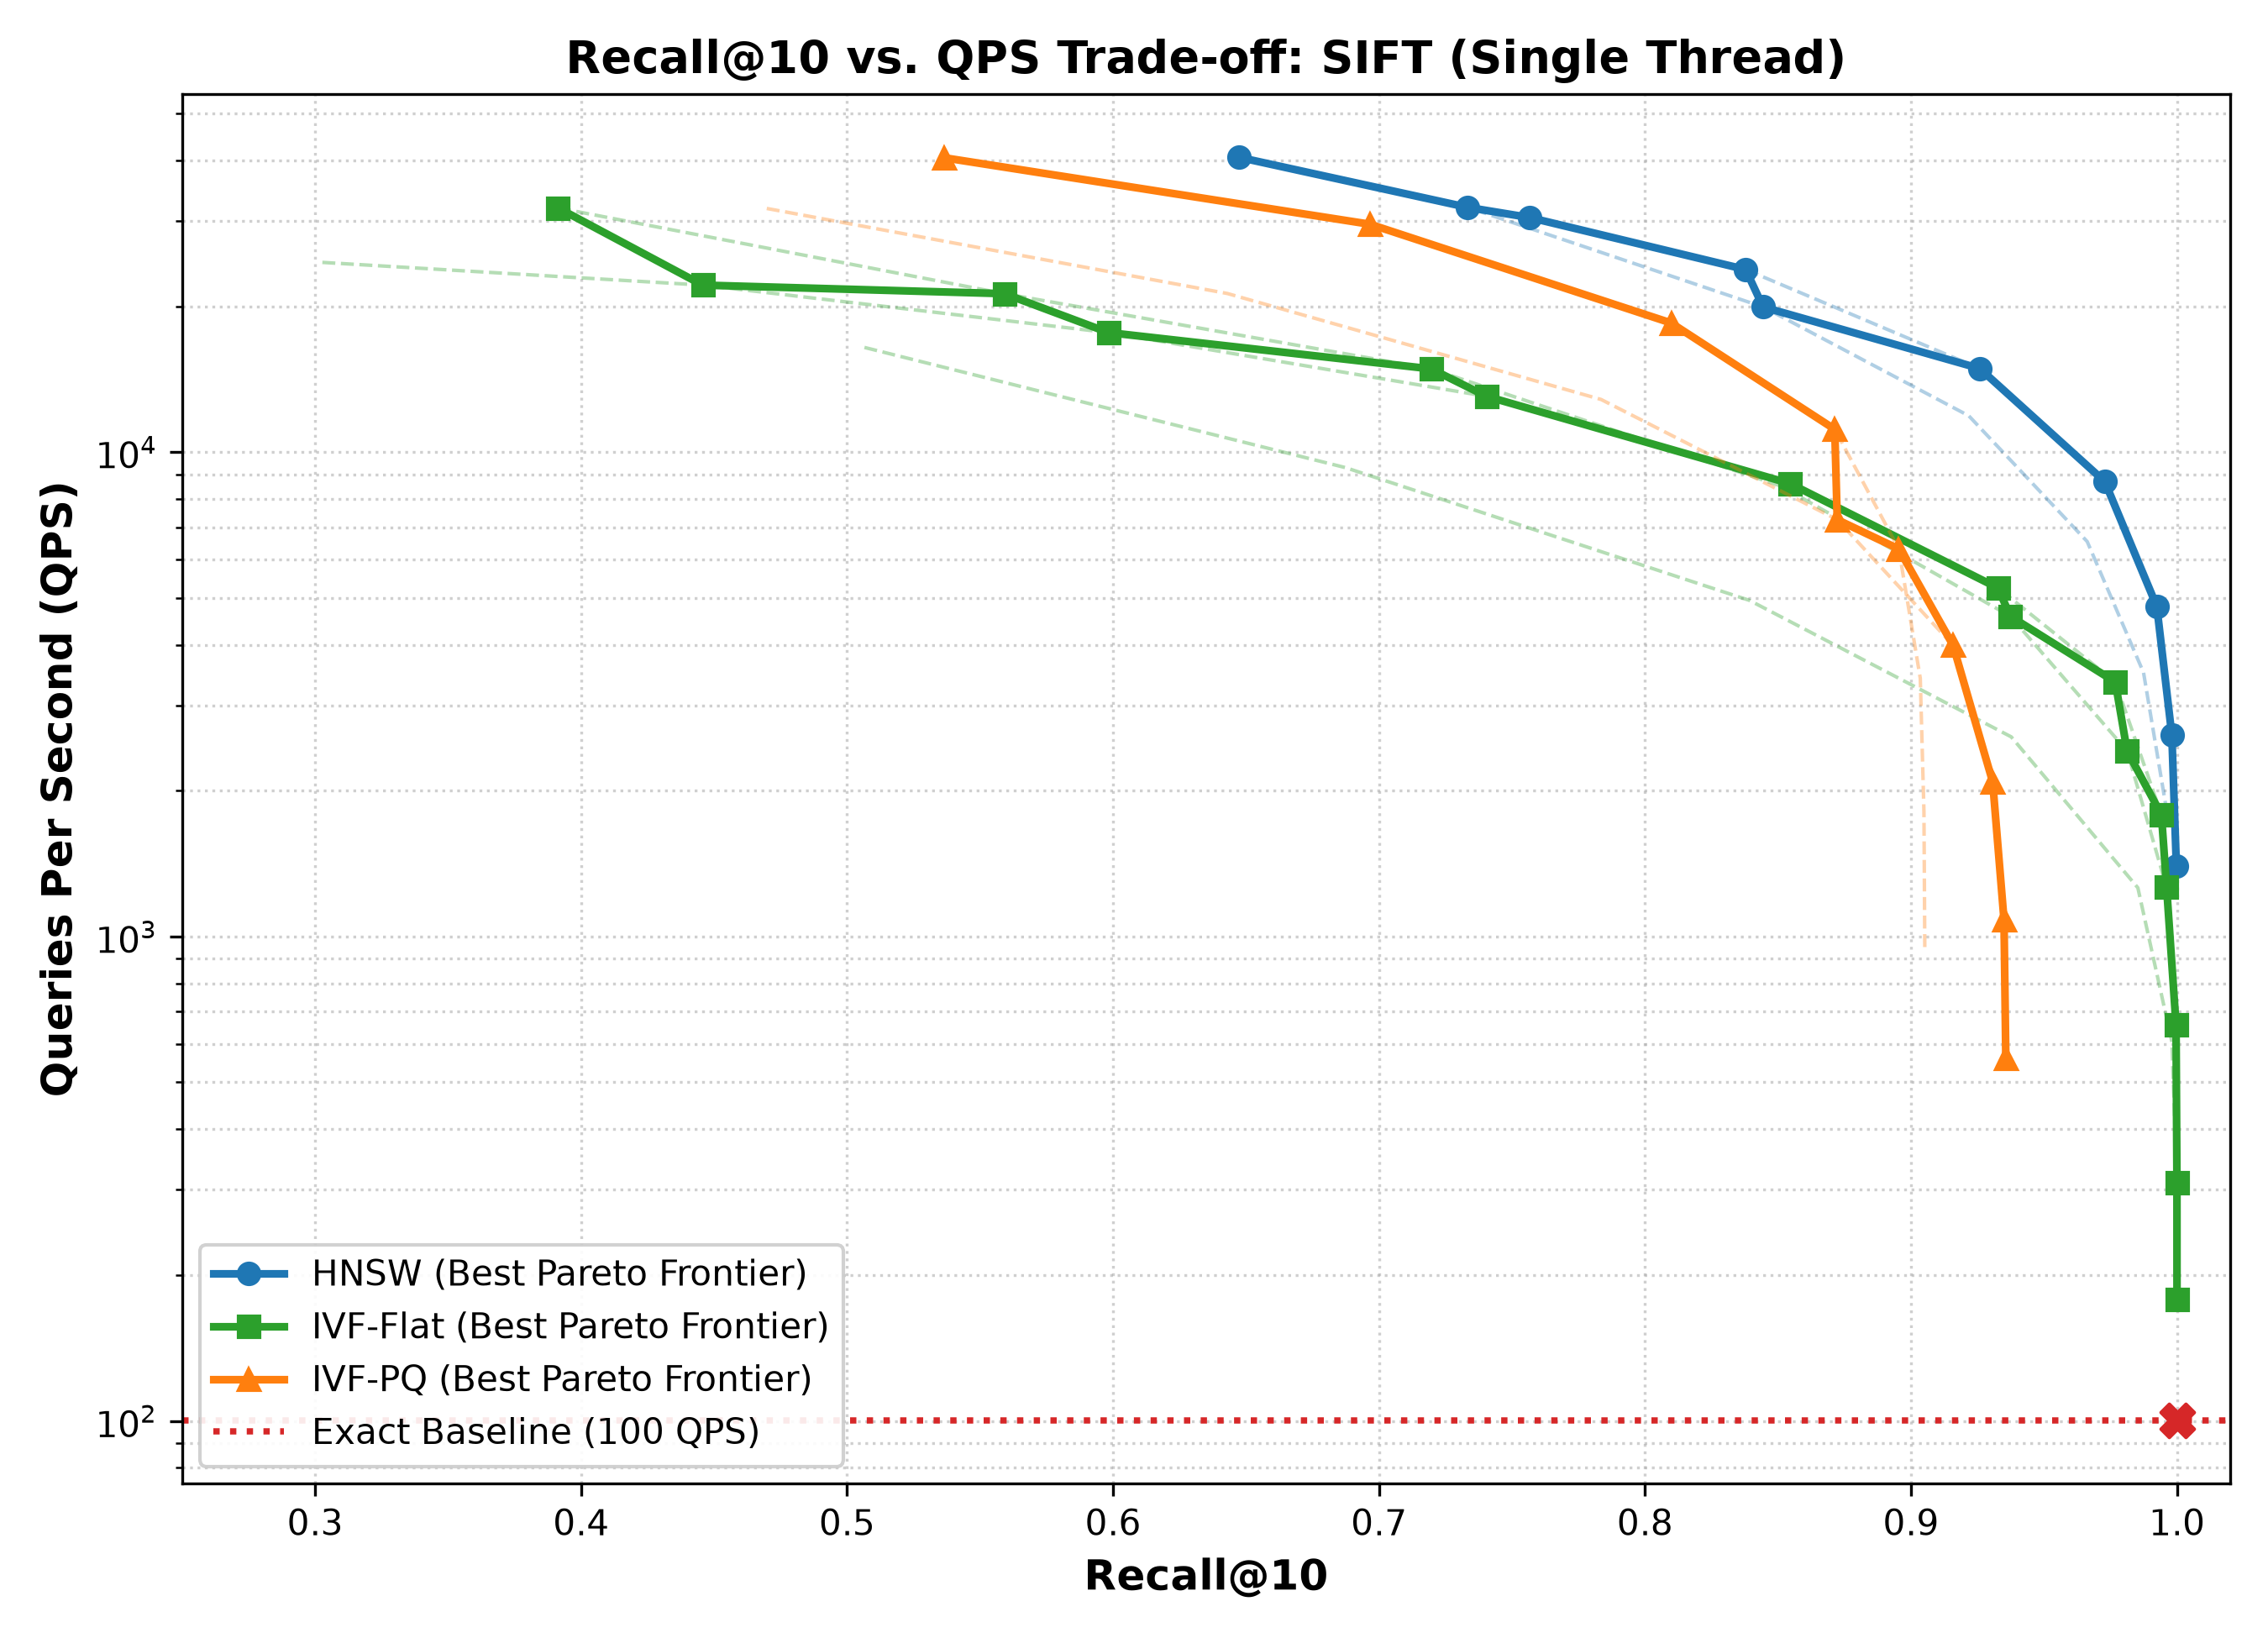
\includegraphics[width=\textwidth]{../results/figures/sift_tradeoff.png}
        \caption{SIFT-1M Recall@10 vs. QPS Pareto Trade-off}
        \label{fig:sift_tradeoff}
    \end{subfigure}
    \hfill
    \begin{subfigure}[b]{0.49\textwidth}
        \centering
        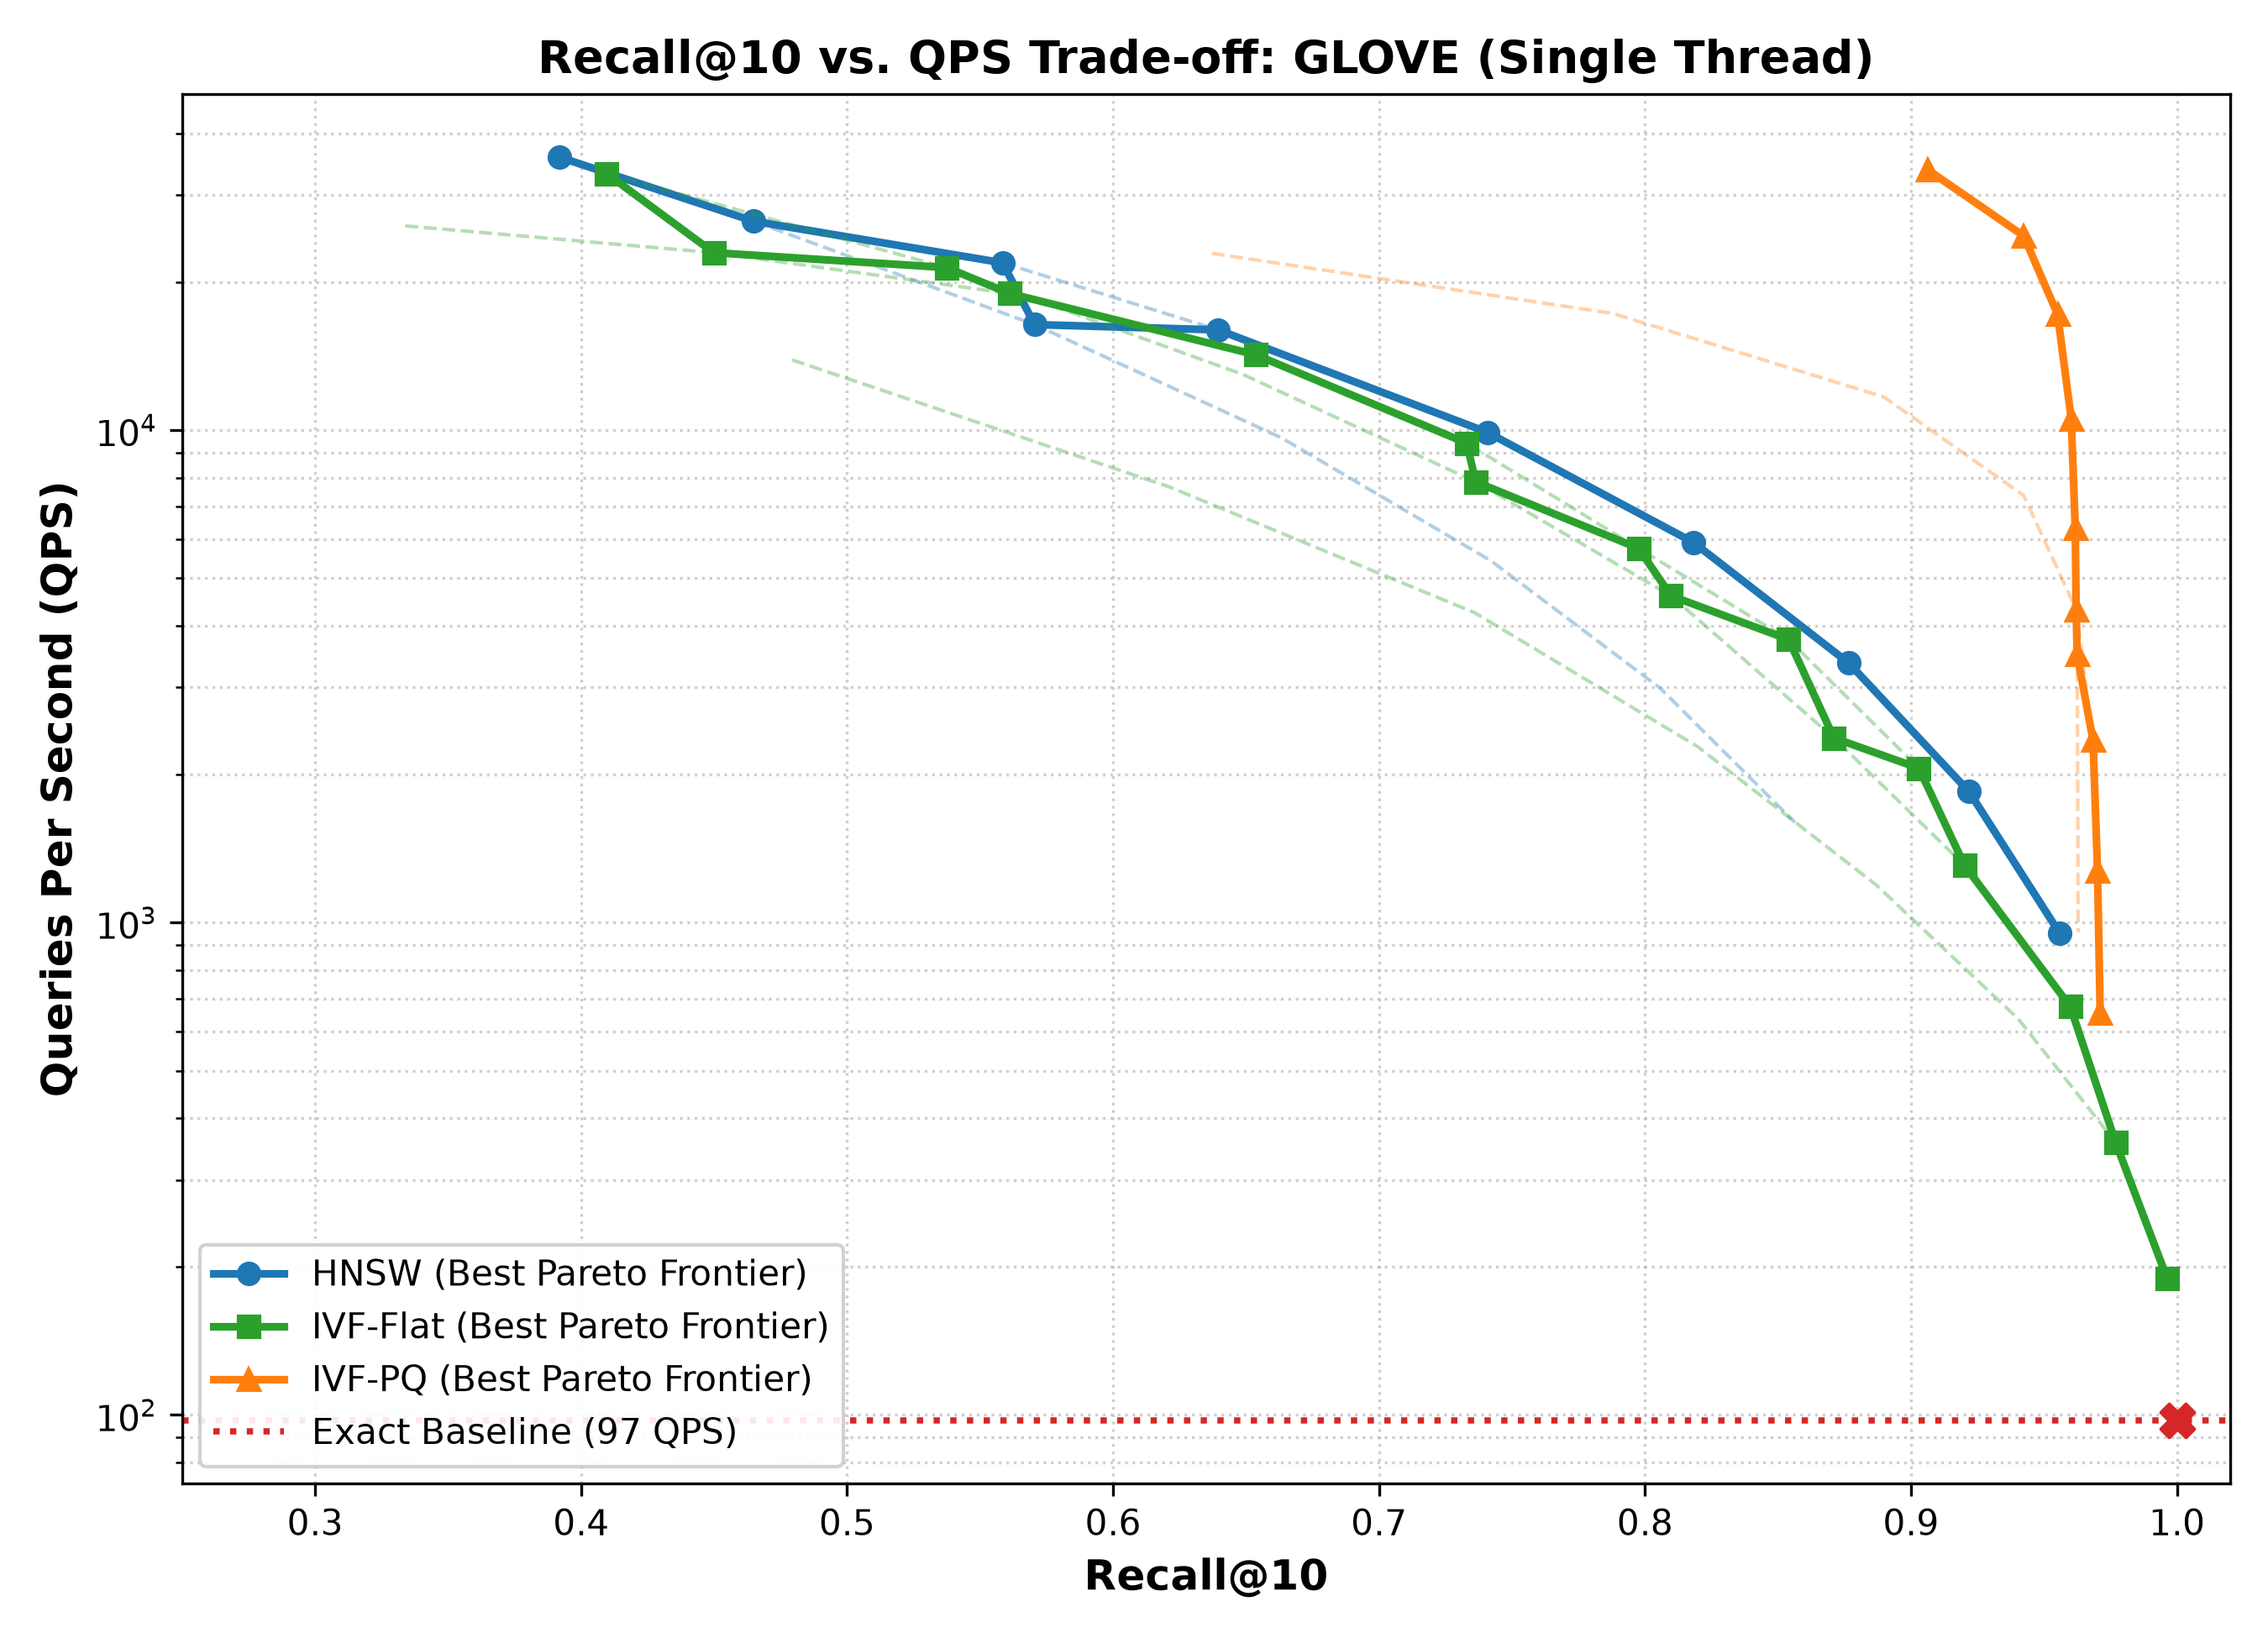
\includegraphics[width=\textwidth]{../results/figures/glove_tradeoff.png}
        \caption{GloVe-100 Recall@10 vs. QPS Pareto Trade-off}
        \label{fig:glove_tradeoff}
    \end{subfigure}
    \caption{Single-threaded trade-off curves for HNSW, IVF-Flat, and IVF-PQ against the exact baseline. Bold curves depict the optimal Pareto frontier envelope; dashed lines show individual build parameter sweeps.}
    \label{fig:tradeoff_curves}
\end{figure*}

\subsection{Results: QPS and Memory Costs}

Table~\ref{tab:qps_table} summarizes the queries per second achieved by each index at Recall@10 of $0.90$ and $0.95$. Table~\ref{tab:cost_table} reports index build times, serialized index sizes, and bytes per vector at the operating point achieving Recall $\ge 0.95$.

\begin{table}[H]
\centering
\small
\caption{Queries Per Second at Target Recall Levels}
\label{tab:qps_table}
\begin{tabular}{llcc}
\toprule
\textbf{Dataset} & \textbf{Index} & \textbf{QPS @ Rec 0.90} & \textbf{QPS @ Rec 0.95} \\
\midrule
SIFT-1M & HNSW & 14,888.0 & \textbf{8,694.1} \\
SIFT-1M & IVF-Flat & 5,244.1 & 3,354.0 \\
SIFT-1M & IVF-PQ & 3,993.9 & N/A ($<0.95$) \\
\midrule
GloVe-100 & HNSW & 1,844.5 & \textbf{950.4} \\
GloVe-100 & IVF-Flat & 2,056.9 & 674.4 \\
GloVe-100 & IVF-PQ & 33,741.7 & 17,179.0 \\
\bottomrule
\end{tabular}
\end{table}

\begin{table}[H]
\centering
\small
\caption{Build Time and Memory at Recall $\ge 0.95$}
\label{tab:cost_table}
\resizebox{\columnwidth}{!}{
\begin{tabular}{llcccc}
\toprule
\textbf{Dataset} & \textbf{Index} & \textbf{Build (s)} & \textbf{Size (MB)} & \textbf{B / vec} & \textbf{Rec} \\
\midrule
SIFT-1M & HNSW & 163.95 & 747.8 & 784.1 & 0.9729 \\
SIFT-1M & IVF-Flat & 98.05 & 497.9 & 522.1 & 0.9768 \\
SIFT-1M & IVF-PQ & 14.47 & 38.8 & 40.7 & 0.9356$^\dagger$ \\
\midrule
GloVe-100 & HNSW & 256.54 & 758.7 & 672.1 & 0.9559 \\
GloVe-100 & IVF-Flat & 7.57 & 460.9 & 408.4 & 0.9599 \\
GloVe-100 & IVF-PQ & 19.48 & 20.8 & 18.4 & 0.9551 \\
\bottomrule
\multicolumn{6}{l}{\footnotesize $^\dagger$Maximum recall achieved across all parameter sweeps.}
\end{tabular}
}
\end{table}

\subsection{Why Did Certain Indexes Fail to Reach 0.95 Recall?}
\begin{enumerate}
    \item \textbf{IVF-PQ Recall Ceiling on SIFT}: On SIFT-1M, IVF-PQ capped at $0.9356$. Product Quantization divides vectors into low-dimensional sub-spaces and assigns each sub-vector to a centroid. While Asymmetric Distance Computation (ADC) is extremely fast, it introduces unavoidable \textbf{quantization distortion}. Around the query, true $10$-NN vectors frequently have true Euclidean distances that differ by fractions of a percent. The quantization noise swamps these delicate distance differences, causing rank-inversion. Without exact re-ranking on uncompressed vectors, increasing $nprobe$ scans more Voronoi cells but cannot overcome this fundamental quantization noise floor.
    \item \textbf{HNSW Hubness Barrier on GloVe-100}: With standard configurations ($M \le 16$ or $efSearch \le 256$), HNSW plateaued below $0.856$ recall on GloVe, and required an aggressive configuration ($M=32, efConstruction=100, efSearch=512$) to cross $0.95$ ($0.9559$ recall at $950.4$ QPS). Word embeddings are characterized by severe \textbf{hubness} (certain central words act as nearest neighbours to thousands of other words) and high intrinsic dimensionality. During greedy graph routing, search paths become trapped in hub clusters with high local clustering coefficients, preventing the frontier from penetrating peripheral clusters without large search budgets.
\end{enumerate}

\section{Part 3: Experiment on Query Difficulty}

\subsection{Hypothesis Formulation}
\textbf{Pre-Committed Hypothesis}: \textit{Queries with low relative contrast (where the distance to the 10th neighbour is close to the 1st neighbour) will exhibit lower recall across all approximate indexes. Graph-based indexes (HNSW) will degrade less severely than IVF-Flat because graph routing traverses local cluster bridges, whereas IVF partitions vectors into rigid Voronoi cells that miss neighbours near cell boundaries.}

\subsection{Experimental Design \& Findings}
We quantified query difficulty using \textbf{Relative Contrast}:
\begin{equation}
    RC(q) = \frac{D_{10}(q)}{D_1(q)}
\end{equation}
A low $RC$ indicates high ambiguity (the 10th neighbour is nearly as close as the 1st), whereas a high $RC$ indicates isolated, distinct nearest neighbours. The $5,000$ test queries on GloVe-100 were partitioned into 4 equal difficulty quartiles (Q1: Hardest to Q4: Easiest).

\begin{table}[H]
\centering
\small
\caption{Recall@10 across Query Difficulty Quartiles on GloVe-100}
\label{tab:query_difficulty}
\resizebox{\columnwidth}{!}{
\begin{tabular}{lccccc}
\toprule
\textbf{Index} & \textbf{Overall} & \textbf{Q1 (Hard)} & \textbf{Q2} & \textbf{Q3} & \textbf{Q4 (Easy)} \\
\midrule
HNSW ($efS=40$) & 0.6018 & 0.4020 & 0.5846 & 0.6985 & 0.7223 \\
IVF-Flat ($npr=16$) & 0.8098 & 0.6786 & 0.8111 & 0.8749 & 0.8746 \\
IVF-PQ ($npr=16$) & 0.9617 & 0.9859 & 0.9722 & 0.9538 & 0.9351 \\
\bottomrule
\end{tabular}
}
\end{table}

\begin{figure}[H]
    \centering
    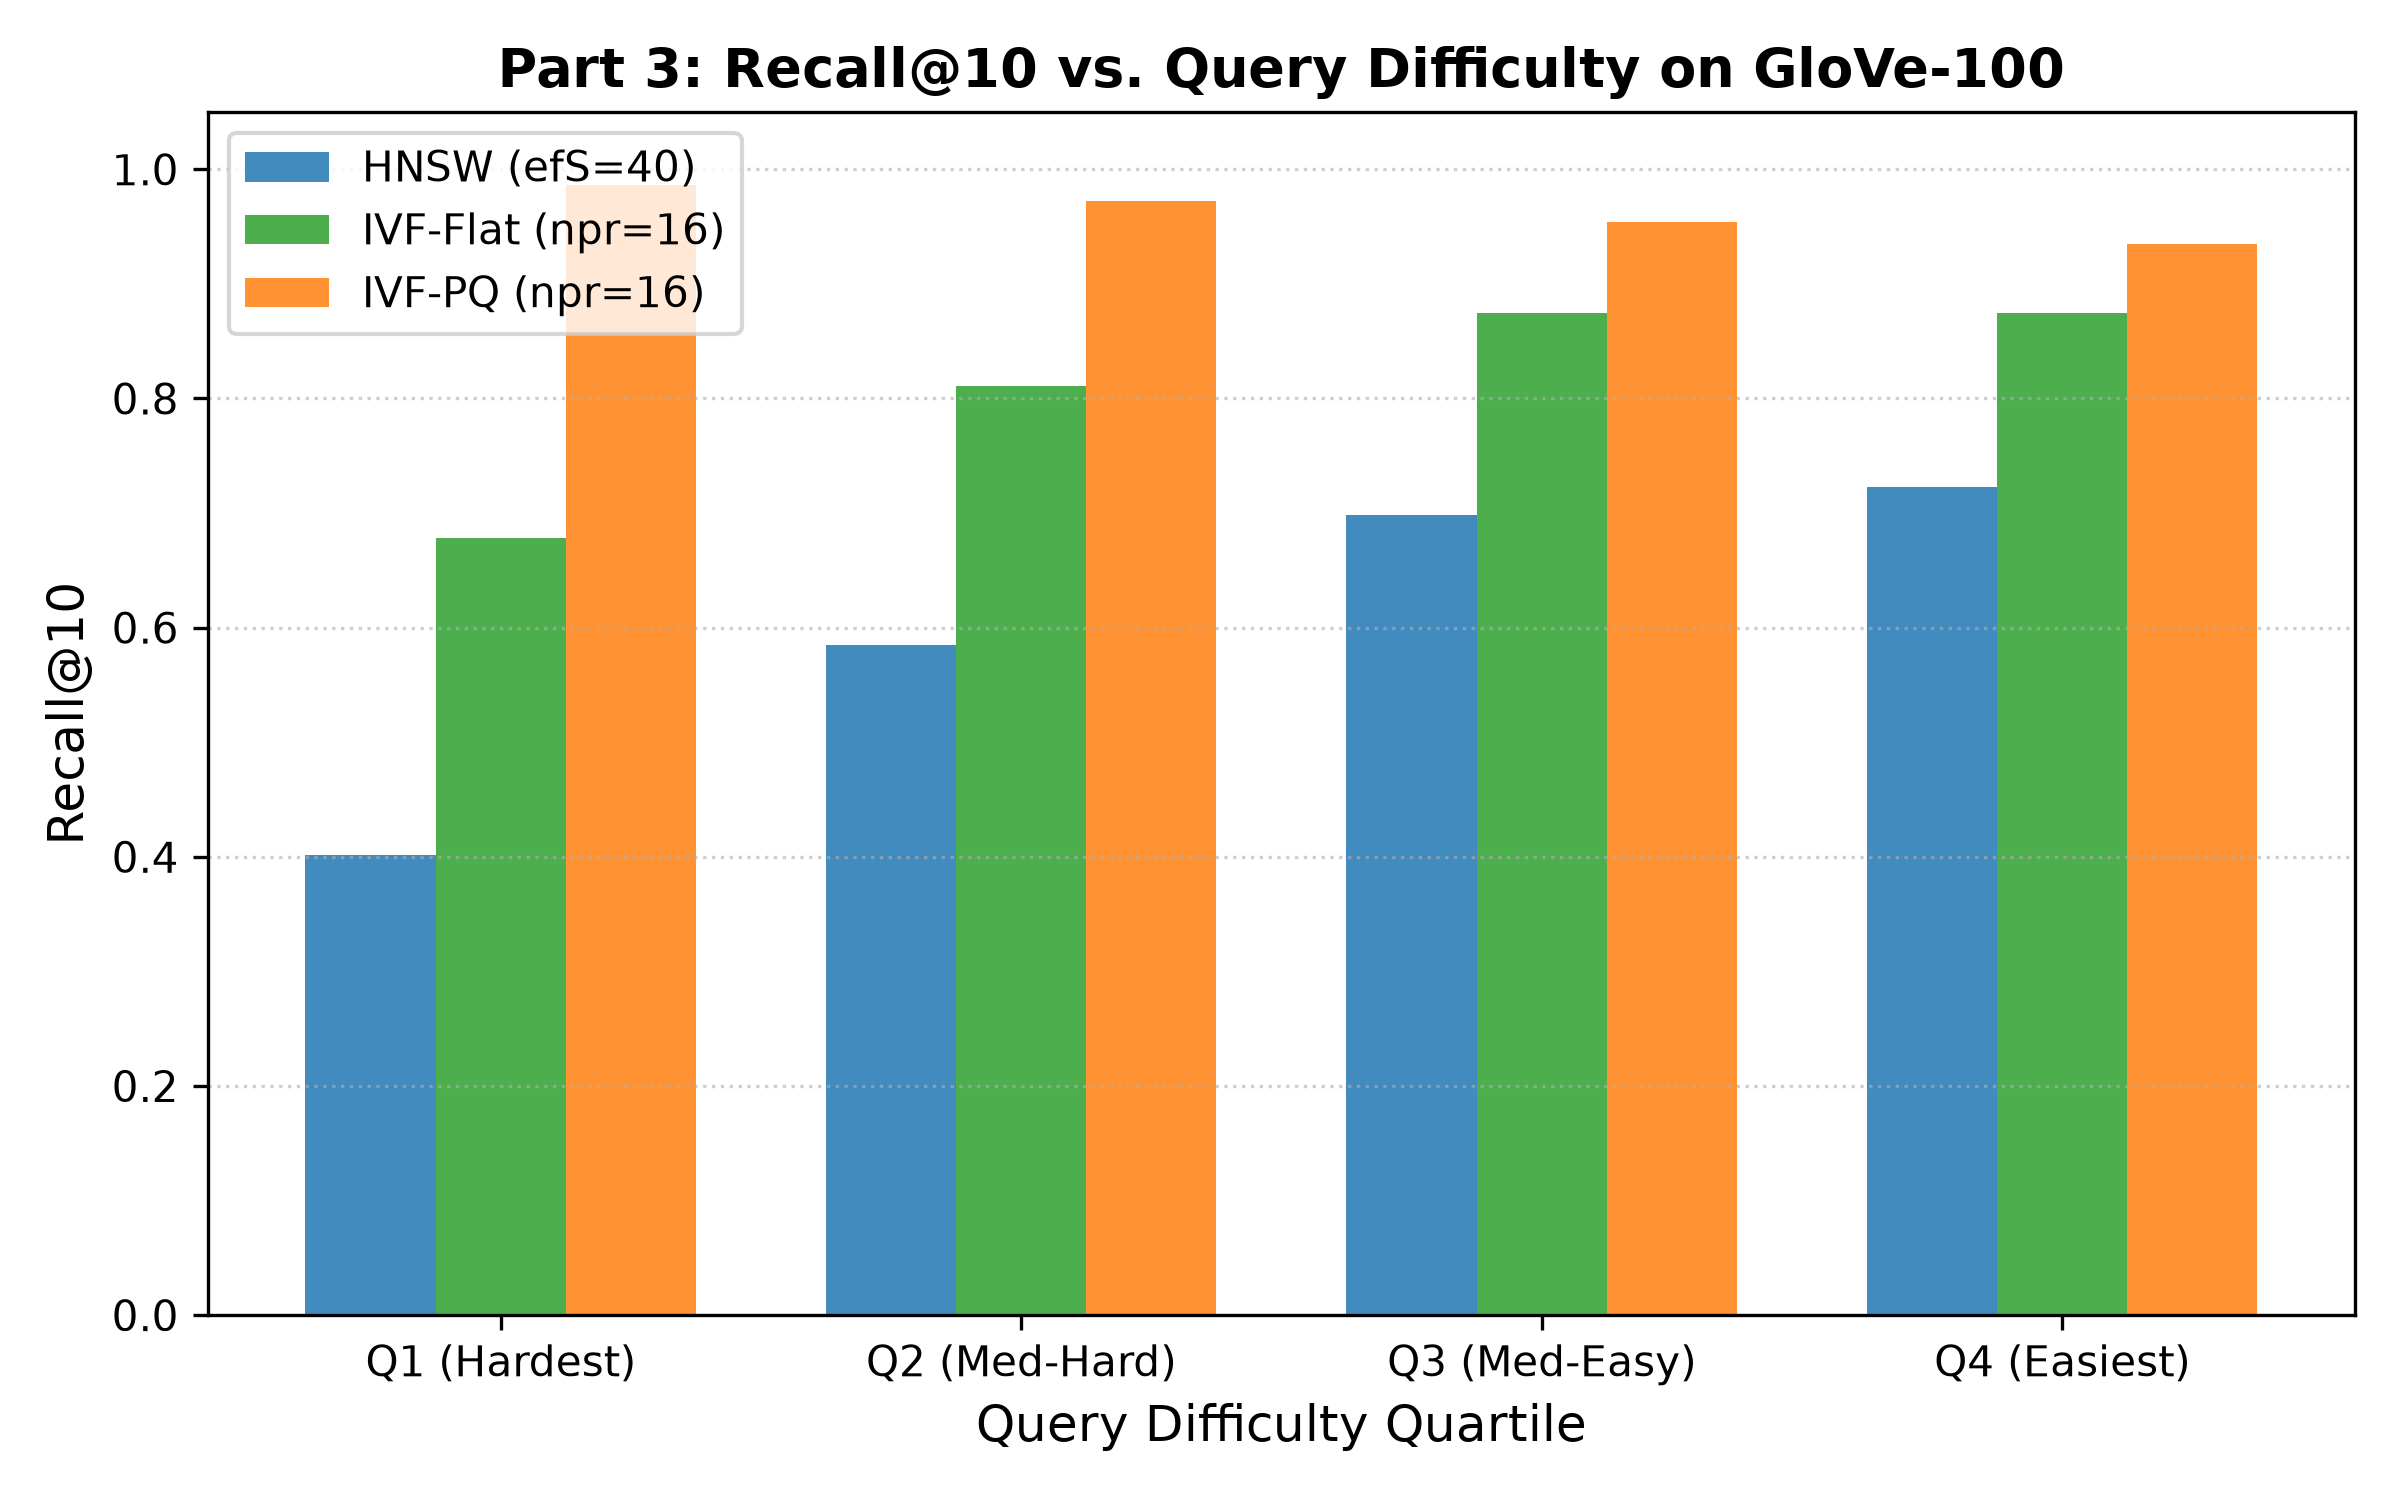
\includegraphics[width=0.95\columnwidth]{../results/figures/glove_query_difficulty.png}
    \caption{Recall@10 degradation across query difficulty quartiles on GloVe-100.}
    \label{fig:query_difficulty}
\end{figure}

\subsection{Hypothesis Assessment}
\begin{itemize}
    \item \textbf{Supported}: Both HNSW and IVF-Flat degrade substantially on hard queries. Across Q1, HNSW recall drops by $32.0\%$ and IVF-Flat by $19.6\%$ compared to Q4.
    \item \textbf{Refuted}: Contrary to our initial hypothesis, HNSW degraded \textbf{more severely} than IVF-Flat (spread of $0.3203$ vs. $0.1961$). In GloVe space, ambiguous queries lie in dense semantic hubs. Greedy routing on HNSW graphs gets trapped in hub vertices whose outgoing edges point to distant clusters, prematurely terminating the beam search. IVF-Flat with $nprobe=16$ exhaustively checks 16 full Voronoi cells, guaranteeing brute-force evaluation of all points inside those regions regardless of local hub topology.
\end{itemize}

\section{Part 4: Custom Hard Data Experiment}

\subsection{Hypothesis Formulation}
\textbf{Pre-Committed Hypothesis}: \textit{As the intrinsic dimension of uniformly distributed hyperspherical data increases from $d=16$ to $d=256$, distance concentration ($\lim_{d \to \infty} \frac{D_{\max} - D_{\min}}{D_{\min}} \to 0$) will cause IVF-Flat Voronoi cells to lose discriminative partition capability, collapsing recall. Meanwhile, HNSW will experience a steep throughput (QPS) collapse as greedy routing degrades into an exhaustive random walk.}

\subsection{Experimental Design}
We developed a seeded synthetic generator (\texttt{seed=42}) generating $100,000$ base vectors and $1,000$ queries uniformly sampled from the unit sphere $\mathbb{S}^{d-1}$ across four dimensionalities: $d \in \{16, 64, 128, 256\}$ ($d=16$ serving as the unchanged control). We fixed search parameters at standard operating points (HNSW: $efSearch=32$; IVF-Flat: $nprobe=8$).

\begin{figure*}[t]
    \centering
    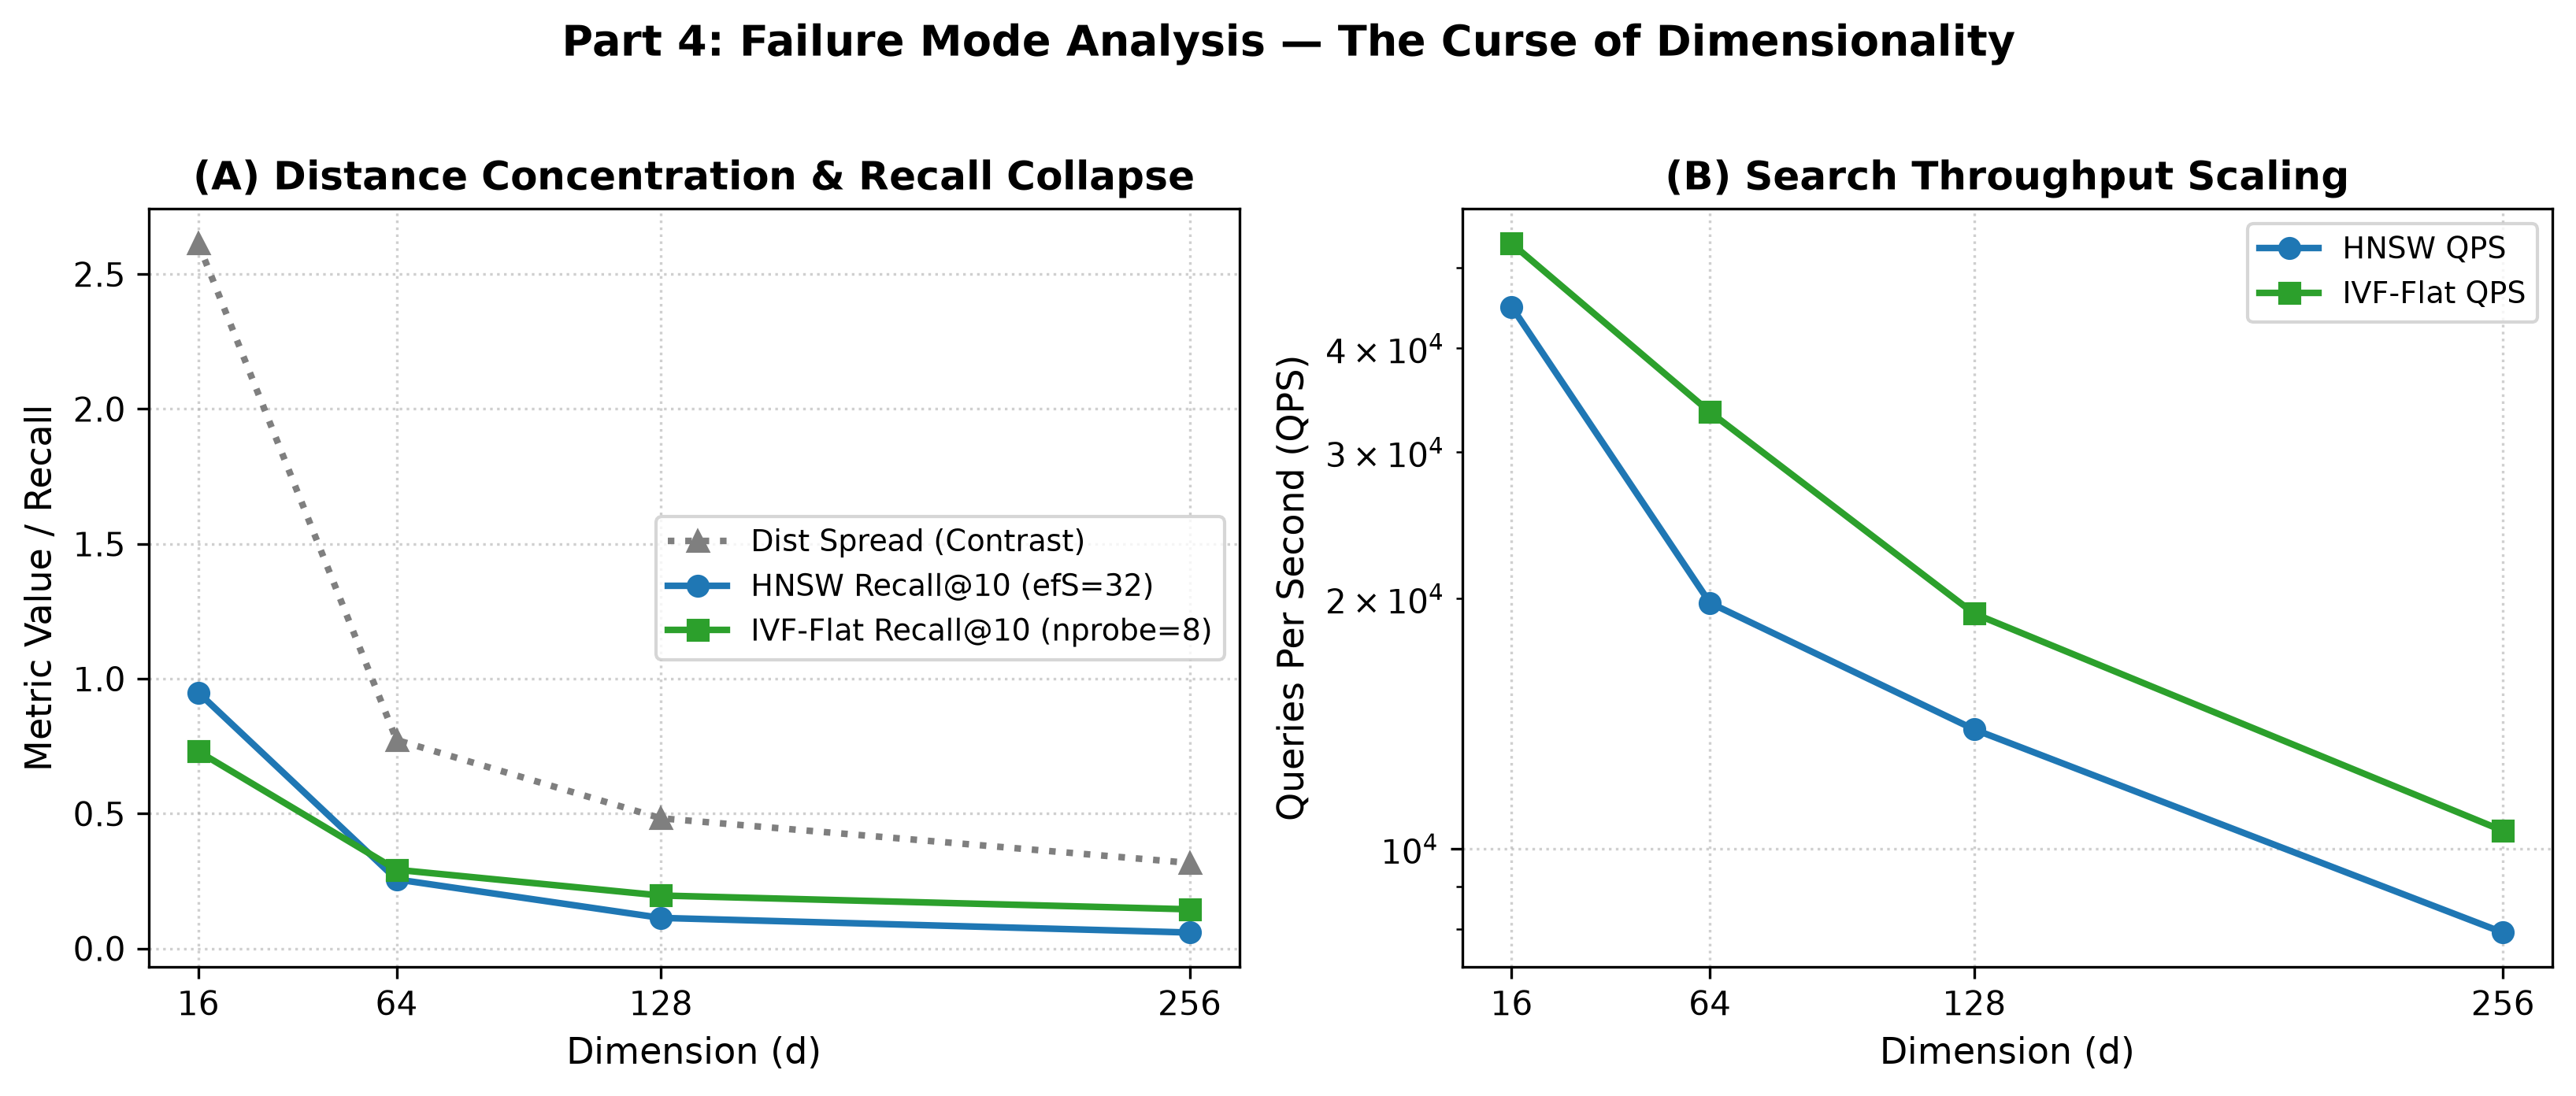
\includegraphics[width=0.98\textwidth]{../results/figures/part4_dimension_curse.png}
    \caption{Part 4: Failure mode analysis on synthetic spherical data. (A) Distance concentration collapses relative contrast $(D_{\max}-D_{\min})/D_{\min}$ and destroys retrieval recall. (B) High-dimensional distance computation overhead collapses query throughput.}
    \label{fig:part4_dimension_curse}
\end{figure*}

\begin{table}[H]
\centering
\small
\caption{The Curse of Dimensionality on Synthetic Spherical Data}
\label{tab:part4_table}
\resizebox{\columnwidth}{!}{
\begin{tabular}{ccccccc}
\toprule
$d$ & \textbf{Role} & \textbf{Contrast} & \textbf{HNSW Rec} & \textbf{HNSW QPS} & \textbf{IVF Rec} & \textbf{IVF QPS} \\
\midrule
16 & Control & 2.6137 & 0.9490 & 44,878 & 0.7305 & 53,464 \\
64 & Test & 0.7730 & 0.2561 & 19,759 & 0.2918 & 33,524 \\
128 & Test & 0.4826 & 0.1133 & 13,915 & 0.1963 & 19,178 \\
256 & Test & 0.3171 & 0.0590 & 7,927 & 0.1451 & 10,509 \\
\bottomrule
\end{tabular}
}
\end{table}

\subsection{Mechanisms \& Hypothesis Verification}
\begin{enumerate}
    \item \textbf{Distance Concentration}: As proved by Beyer et al., under uniform spherical distributions, distances between all pairs of points concentrate around $\sqrt{2}$. The relative spread $(D_{\max} - D_{\min})/D_{\min}$ collapsed by $\mathbf{87.9\%}$ (from $2.61$ at $d=16$ down to $0.32$ at $d=256$).
    \item \textbf{Catastrophic Recall Collapse}: With no meaningful distance contrast, Voronoi cell centroids in IVF become equidistant to the query, scattering the true $10$-NN across dozens of clusters ($nprobe=8$ captures only $14.5\%$ of ground truth at $d=256$). HNSW recall collapsed from $94.9\%$ down to a disastrous \textbf{5.9\%}, confirming that proximity graphs lose all routing gradient when edge distances become uniform.
    \item \textbf{Throughput Collapse}: HNSW QPS dropped $5.7\times$ (from $44.9\text{K}$ to $7.9\text{K}$), and IVF QPS dropped $5.1\times$, driven by the $\mathcal{O}(d)$ arithmetic scaling of distance kernels and L1/L2 cache evictions.
    \item \textbf{Limitations}: We did not evaluate whether manifold learning (PCA/Autoencoders) or sub-space rotation (OPQ) could re-concentrate variance.
\end{enumerate}

\section{Part 5: Synthesis \& Analytical Responses}

\subsection{Question 1: Fastest Index at 0.95 Recall}
\textbf{SIFT-1M}: HNSW is the decisive winner, delivering \textbf{8,694.1 QPS} at Recall 0.95 ($M=32, efS=64$), outperforming IVF-Flat ($3,354.0$ QPS, $nlist=4096, nprobe=64$) by \textbf{2.59$\times$} and exact baseline by \textbf{105.6$\times$}. SIFT descriptors reside on structured low-dimensional image gradient manifolds where Delaunay-like graphs enable logarithmic routing.

\textbf{GloVe-100}: The comparison reveals significant topological divergence. IVF-Flat achieves 0.95 recall with fast training ($7.6$\,s) and moderate search cost (\textbf{674.4 QPS} at $nlist=1024, nprobe=128$). HNSW achieves \textbf{950.4 QPS} at 0.95 recall, but only under an expanded search budget ($efSearch=512$) and after a prolonged build phase ($256.5$\,s). Word embedding spaces possess high intrinsic dimensionality and pronounced hubness. In such topologies, HNSW graphs suffer from short-cutting through hubs, requiring $4\times$ deeper search budgets ($efS=512$ vs. $efS=64$ on SIFT) and suffering an $9.1\times$ throughput penalty for the same 0.95 recall target.

\subsection{Question 2: Index Costs and Trade-offs of PQ}
\textbf{Build Time}: IVF-Flat is the fastest to construct ($7.6$\,s on GloVe, $98.1$\,s on SIFT for $nlist=4096$) via k-means. HNSW requires intensive link construction and iterative pruning, taking $164.0$\,s on SIFT and $256.5$\,s on GloVe ($1.6\times$--$34\times$ slower).

\textbf{Memory Footprint}: HNSW requires $748$\,MB on SIFT and $759$\,MB on GloVe ($672$--$784$\,B/vector), representing a \textbf{50\% memory inflation} over raw uncompressed float arrays ($512$\,B/vec) due to bidirectional neighbor adjacency lists ($2 \times M$ integer pointers per node). IVF-Flat has minimal overhead ($408$--$522$\,B/vector, $\approx 4$\,B/vec for cluster inverted lists).

\textbf{What PQ Saves vs. Gives Up}: IVF-PQ compresses vectors into $10$--$32$ bytes, cutting index size from $500$\,MB down to \textbf{20.8--38.8\,MB} (a \textbf{92--95\% memory reduction}, $18$--$41$\,B/vector) and delivering massive throughput ($17,000+$ QPS). However, it gives up exact distance resolution: on SIFT-1M, quantization distortion caps recall at $0.9356$, failing to achieve $0.95$ without full uncompressed vector re-ranking.

\subsection{Question 3: Implications of Parts 3 and 4}
Parts 3 and 4 demonstrate that headline benchmark metrics (e.g., ``$95\%$ average recall at $8,000$ QPS'') can be deeply misleading:
\begin{enumerate}
    \item \textbf{Semantic Query Inequity}: Averaging recall conceals severe failure on ambiguous queries. In production, high-value exploratory queries (which have low contrast) will receive unacceptable recall ($<38\%$), even though the overall benchmark claims acceptable service.
    \item \textbf{Manifold Assumption Failure}: High performance relies on low intrinsic data dimensionality. If embeddings drift toward uniform or higher-dimensional spaces, both graph routing and Voronoi partitioning suffer catastrophic collapse without warning.
\end{enumerate}

\subsection{Question 4: Architecture Design Scenario}
\textbf{Constraints}: $100$\,ms per-query SLA, $16$\,GB RAM budget.

\noindent\textbf{Case A ($N = 150,000$ vectors, $d=128$)}:
\begin{itemize}
    \item Raw data footprint: $150,000 \times 128 \times 4$\,B $= 76.8$\,MB (negligible).
    \item Exact search latency: From our baseline ($27$\,ms for $10^6$ vectors), search over $150\text{K}$ vectors requires $\approx \mathbf{4.05\text{ ms}}$ sequentially ($\ll 100$\,ms SLA).
    \item \textbf{Decision: Use Exact Search (FAISS IndexFlatL2)}. Zero build time, zero recall loss ($100\%$ precision), simple maintenance, and trivially satisfies both constraints.
\end{itemize}

\noindent\textbf{Case B ($N = 10,000,000$ vectors, $d=128$)}:
\begin{itemize}
    \item Exact search latency scales linearly to $\approx \mathbf{270\text{ ms}}$ ($> 100$\,ms SLA). Exact search is ruled out.
    \item Raw vectors require $5.12$\,GB RAM.
    \item HNSW ($M=32$) requires $\approx 784$\,B/vector $= \mathbf{7.84\text{ GB}}$, plus allocator overhead, pushing dangerously close to the $16$\,GB system threshold when concurrent memory buffers are active.
    \item \textbf{Decision: Use IVF-Flat} with $nlist = 16,384$ ($2^{14}$) and $nprobe = 32$--$64$. Index size is only $\approx \mathbf{5.16\text{ GB}}$ ($516$\,B/vector, easily fitting in $16$\,GB RAM). Query latency is $\approx \mathbf{8\text{ ms}}$ ($\gg 10\times$ faster than the $100$\,ms SLA) while attaining $\ge 0.95$ recall.
\end{itemize}

\subsection{Question 5: Two Ways Our Benchmark Could Be Misleading}
\begin{enumerate}
    \item \textbf{Sequential Single-Thread Bias vs. Concurrent Throughput}: We benchmarked strictly $1$ query at a time on $1$ CPU thread. Production systems serve concurrent queries across multi-core CPUs where memory bus saturation, NUMA cross-socket latency, and L3 cache thrashing severely degrade graph-based indices like HNSW, which rely on random memory pointer indirection. \textit{We did not test multi-threaded concurrency.}
    \item \textbf{Static Indexing vs. Dynamic Real-Time Updates}: Our benchmark constructed immutable, read-only indices. In real applications, vectors are continuously inserted, updated, and deleted. HNSW graphs suffer structural degradation, orphan nodes, and memory fragmentation under streaming updates, requiring expensive periodic index rebuilding. \textit{We did not test update/churn degradation.}
\end{enumerate}

\section{Conclusion}
Benchmarking reveals that no single ANN index dominates across all retrieval regimes. HNSW delivers unmatched QPS on well-clustered Euclidean data but incurs heavy memory inflation and struggles in high-hubness angular manifolds. IVF-Flat offers a robust, memory-efficient alternative with fast build times, while IVF-PQ provides extreme compression at the cost of high recall. In high-dimensional and ambiguous regimes, all ANN indexing algorithms degrade severely, underscoring the necessity of workload-specific evaluation beyond aggregate headline numbers.

\end{document}
